\documentclass[]{beamer}
\usetheme{Boadilla}

\usepackage{amsmath}
\usepackage{amssymb}
\usepackage{bm}
\usepackage{graphicx}
\beamerdefaultoverlayspecification{<+->}

\title{Lab 8: More on Regression Discontinuity}
\subtitle{Causal Inference}
\author{Chanhyuk Park and Xiangyu Song}
\institute{Washington University in St. Louis}
\date{}

\begin{document}
\begin{frame}
    \titlepage
\end{frame}

\begin{frame}{Topics}
    \begin{enumerate}[<*>]
        \item Bandwidth Selection
        \vspace{0.3cm}
        \item Discrete Running Variables
        \vspace{0.3cm}
        \item Density Tests
    \end{enumerate}
\end{frame}

\begin{frame}{Bandwidth Selection: The Bias-Variance Tradeoff}
    \begin{itemize}
        \item How should we select the bandwidth ($h$)?
        \item One simple way is to find the one that minimizes the MSE
            $$ 
                \text{MSE}(\hat{\tau}) = \mathbb{E}[(\hat{\tau} - \tau)^2] = \text{Bias}(\hat{\tau})^2 + \text{Var}(\hat{\tau}) 
            $$
        \item Let's see how Bias and Variance look like in RD setting!
            \vspace{1cm}
        \item Variance is proportional to the inverse of the sample size $N$, and in RD setting, the local sample size is proportional to $nh$:
            $$
                Var(\hat{\tau}) \propto \frac{1}{nh}
            $$ 
    \end{itemize}
    
\end{frame}

\begin{frame}{Bandwidth Selection: The Bias-Variance Tradeoff}
    \begin{itemize}
        \item Bias is little bit more trickier
        \item Suppose a true treatment effect $m(x) = \mathbb{E}\left[ Y \mid X = x \right]$
        \item Taylor expansion of $m(x)$:
            $$ 
                m(x) = m(c) + m'(c)(x - c) + \frac{1}{2}m''(x - c)^2 + \ldots
            $$
        \item Suppose we fit a local linear regression model $\hat{m}(x) = \beta_0 + \beta_{1}(x - c)$
        \item We can then quantify the bias from the model $\hat{m}(x)$:
            $$
                \text{Bias}(x) = \hat{m}(x) - m(x) \approx \frac{1}{2} m''(c)(x - c)^2
            $$ 
        \item In RD setting, $\left\lvert x - c \right\rvert < h$:
            $$
                \text{Bias}(x) \approx \frac{1}{2} m''(c)h^2
            $$ 
    \end{itemize}
\end{frame}

\begin{frame}{Bandwidth Selection: The Bias-Variance Tradeoff}
    \begin{itemize}
        \item To generalize, MSE in RD looks like this:
            $$
            \begin{aligned}
                MSE(\hat{\tau}) &= &\text{Bias}(\hat{\tau})^2 &+ &\text{Var}(\hat{\tau}) \\ &\propto &(h^{(p + 1)})^2 &+ &\frac{1}{nh} \\
            \end{aligned}
            $$, where $p$ is the order of the model
        \item As $h \to 0$, Bias decreases but variance increases
        \item As $h \to \infty$, Bias increases but variance decreases
        \item Imbens \& Kalyanaraman (2012) suggested $h^*$ that minimizes the formula
        \item Cons: May bias the estimate!
    \end{itemize}
\end{frame}

\begin{frame}{The CCT Solution: Robust Bias-Correction}
    \begin{itemize}
        \item Calonico, Cattaneo, and Titiunik (2014) solved this in two steps:
        \begin{enumerate}
            \item Cancel out bias: Use a Taylor expansion of one order higher to estimate the bias (like we did) and subtract the estimated bias first
            \item Subtracting the bias adds noise $\to$ New SE
            $$ \text{Var}(\hat{\tau}_{BC}) = \text{Var}(\hat{\tau}) + \text{Var}(\widehat{\text{Bias}}) - 2\text{Cov}(\hat{\tau}, \widehat{\text{Bias}}) $$
        \end{enumerate}
        \item No worries we have a package: \texttt{rdrobust}
    \end{itemize}
\end{frame}

\begin{frame}{Discrete Running Variables}
    \begin{itemize}
        \item Standard RD assumes $X_i$ is \textit{continuous} so that we can take limits as $x \to c$ from the left and right
        \item Running variables are often discrete: number of votes
        \item There is no 0.5 vote
            \begin{figure}
                \begin{center}
                    \begin{tabular}{cc}
                        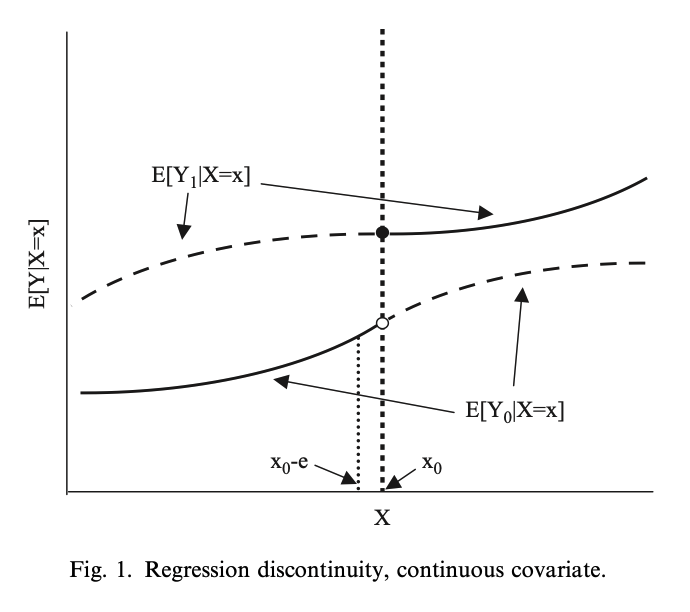
\includegraphics[width=0.4\textwidth]{./leecard1.png} & 
                        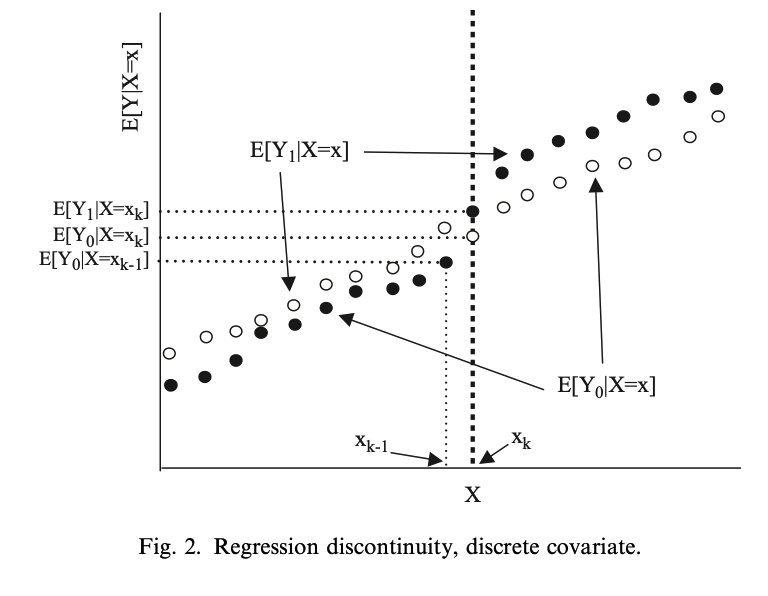
\includegraphics[width=0.4\textwidth]{./leecard2.png} \\
                    \end{tabular}
                \end{center}
            \end{figure}
            

        \item A potential Solution: Lee and Card (2008)
    \end{itemize}
\end{frame}

\begin{frame}{Lee and Card (2008)}
    \begin{itemize}
        \item Because we can't take limits, we \textit{must} assume a model to inter/extrapolate across the gaps
        \item Because we used models to fill the gaps, at each discrete point $g$, we need to account for the model error
            $$ Y_{ig} = f(x_g) + \underbrace{a_g + \epsilon_{ig}}_{\text{Error}} $$
        \item So what? Cluster standard errors by the running variable!
        \item As always, clustered SE may explode if the running variable only have few values (clusters)
        \item Ignore the problem: treat it like a continuous variable
    \end{itemize}
\end{frame}

\begin{frame}{Density Tests: Testing for Sorting}
    \begin{itemize}
        \item If sorting exists, we should see an unnatural "jump" in the number of observations (the density) at the threshold
        \item The Simple Way (McCrary): Histogram
            \begin{enumerate}
                \item Divide $X_i$ into bins
                \item Count the number of units in each bin
                \item Regress the counts on the bin midpoints
            \end{enumerate}
    \end{itemize}
\end{frame}

\begin{frame}{Cattaneo, Jansson, and Ma (2018)}
    \begin{itemize}
        \item Well, binning is subjective!
        \item Let's estimate the density for both sides
        \item Use local polynomial regression to smooth and estimate the CDF
        \item The density is the derivative of the CDF
        \item No headache: \texttt{rddensity}
    \end{itemize}
\end{frame}

\begin{frame}{Practical Advices}
    \begin{itemize}
        \item Use \texttt{rdrobust} to get bias-corrected estimates and robust confidence intervals (data driven bandwidth)
        \item If your running variable is discrete, justify your functional form and cluster standard errors (Lee and Card) or ignore the problem
        \item Use \texttt{rddensity} to prove there is no discontinuity in the density of your running variable.
    \end{itemize}
\end{frame}

\end{document}
